% -*- root: ../main.tex -*-
%!TEX root = ../main.tex
% this file is called up by main.tex
% content in this file will be fed into the main document
% vim:textwidth=80 fo=cqt

To demonstrate that a suitable advancement of the field has indeed been achieved
through  this system  identification exercise,  a comparison  with the  existing
state of the art in reduced  order electrolyte modelling is warranted. Secondly,
to  comprehend its  extent of  validity  and performance  boundaries, the  newly
developed \gls{rom} must also be  pitted against the full-order \gls{p2d} model.
This section  aims to  provide such  a comparative discussion  for two  types of
inputs ---
\begin{enumerate*}[label=\itshape\alph*\upshape)]
    \item constant current inputs
    \item dynamic load profiles
\end{enumerate*}

\subsection{Constant current inputs}

\Cref{fig:tfquadp2dspatialionicconc1C} shows  the spatial distribution  of ionic
concentration  in  the electrolyte  along  cell  thickness  for a  1C  discharge
beginning at \SI{100}{\percent} \gls{soc}. The spatial concentration computed by
each of the three approaches ---
\begin{enumerate*}[label=\roman*)]
    \item the \gls{p2d} model,
    \item the quadratic approximation model and
    \item the newly developed system identification model(s).
\end{enumerate*}

\begin{figure}[!htbp]
    \centering
    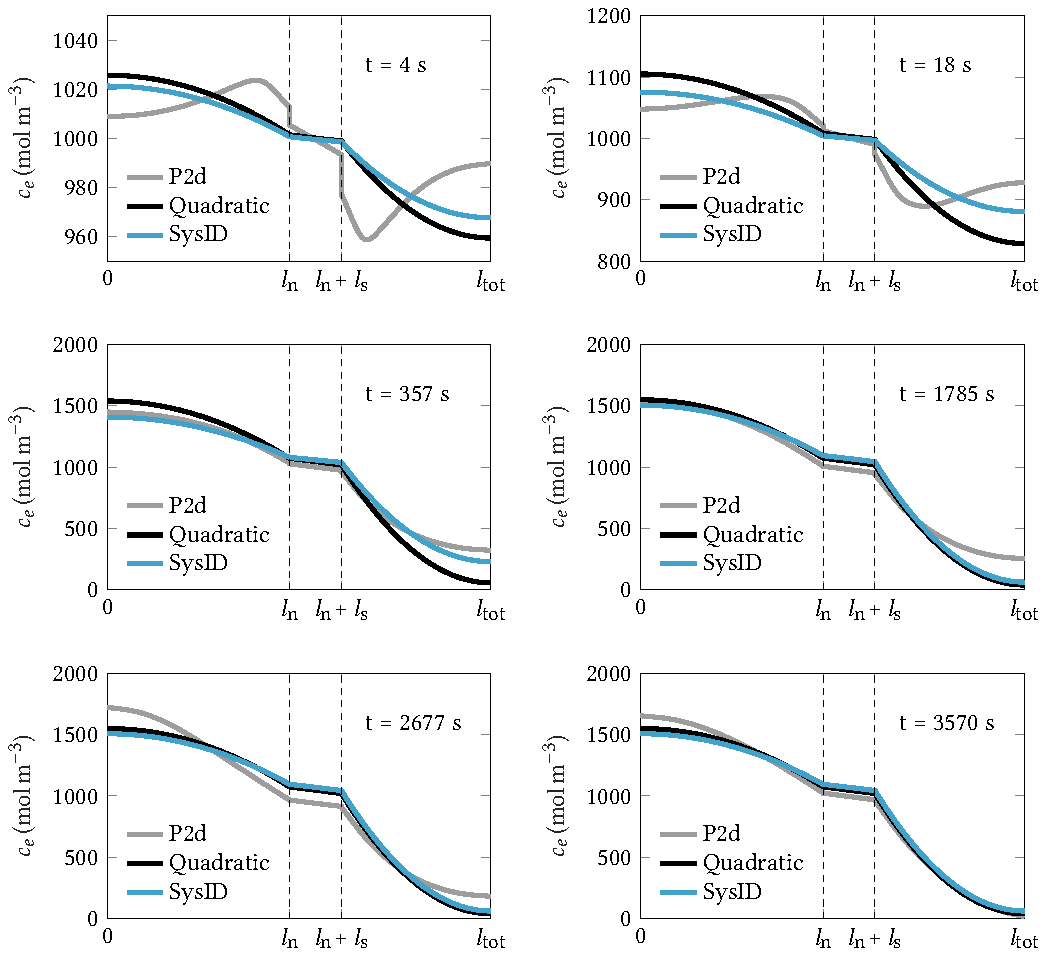
\includegraphics[width=\textwidth]{tf_quadratic_ce_approx_spatial.pdf}
    \caption[Spatial distribution of ionic concentration in
    electrolyte for a 1C discharge computed by the \glsfmtshort{p2d}, quadratic
    approximation \& system identification models]{%
        Spatial distribution of ionic concentration  in electrolyte along cell
        thickness at various  snapshots of  time computed  by each of  the three
        models for  a 1C discharge.  The concentration  profile  computed by
        the  \gls{p2d} model is used as the benchmark reference. The  system
        identification model performs noticeably better than the quadratic
        approximation model during  the initial  transient  while delivering a
        similar performance as a \glsfmtlong{qss} is reached.
}%
\label{fig:tfquadp2dspatialionicconc1C}
\end{figure}

During  the  initial  phase  of   discharge,  the  \gls{p2d}  model  exhibits  a
characteristic inflection point near the  separator interfaces that diffuses out
over time  until a  \gls{qss}. This  is due to  the fact  the reaction  front is
initially established  close to the  separator, and as surface  concentration of
lithium  in particles  near separator  is  depleted, the  reaction starts  moves
further  into the  electrode thickness.  Neither  of the  two \glspl{rom}  under
consideration here  could successfully  capture this  characteristic inflection.
This is  explained by  the fact  that both  of them  use the  standard quadratic
approximation profile for the \emph{spatial}  profile, which means that only one
apex  point is  possible  per  electrode, which  is  pinned  to their  separator
interfaces by design.

During the transient portion of discharge (approximately up to \SI{357}{\second}
as   shown   in~\cref{fig:tfquadp2dspatialionicconc1C}),   the  locus   of   the
concentration  profile computed  by  the newly  developed system  identification
model(s) clearly lies  much closer to the \gls{p2d} model  than that computed by
the  quadratic  approximation model.  After  the  initial transition  phase,  it
appears  that  the  concentration  profile predicted  by  both  the  \glspl{rom}
converge to the \gls{p2d} model's concentration profile.


To obtain  a quantifiable  perspective on  the accuracy  of the  newly developed
model, it  is desirable  to plot  the temporal  evolution of  the concentration,
particularly  at  the  two  current   collector  interfaces.  The  behaviour  of
the  baseline  quadratic approximation  model  in  this regard  was  established
in~\cref{subsubsec:simresultsbaselinequad}.   Therefore  it   is  important   to
ascertain whether a noteworthy improvement  was achieved using the model arrived
at using the system identification procedure.


% although constant current discharge is not important, it provides a glimpse on
% the applicability of the model to dynamic conditions and is a reference
% benchmark. Why is it not possible to use this for dynamic inputs? Explain how
% large concentration gradients are established that deviate away from the
% training profile. So the small-signal approximation used by the discrete-time
% transfer function no longer holds true.
